\documentclass[a4paper,11pt]{article}
\usepackage[T1]{fontenc}
\usepackage{tikz}
\usetikzlibrary{shapes,arrows,chains,decorations.pathreplacing}
\usepackage{xcolor}
\usepackage{amsmath}

\begin{document}

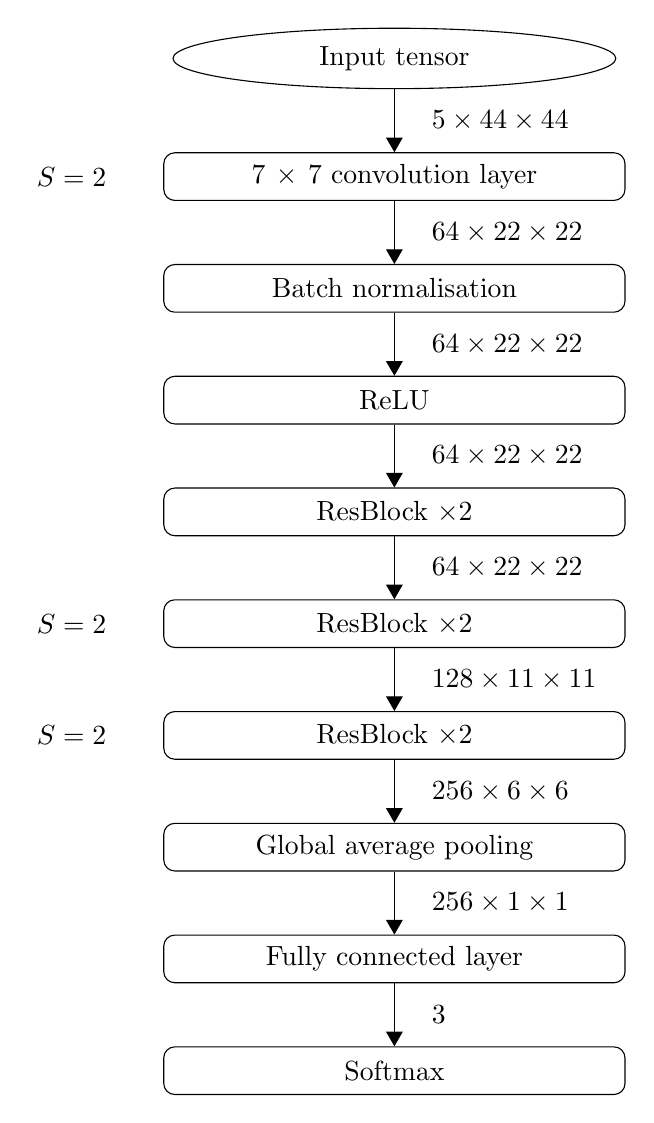
\begin{tikzpicture}[%
    >=triangle 60,
    start chain=going below, 
    node distance=8mm and 6mm,
        every join/.style={norm},
    ]

\tikzset{
  base/.style={draw, on chain, on grid, align=center, minimum height=4ex},
  proc/.style={base, rectangle, text width=16em,rounded corners},
  inpt/.style={base, ellipse,minimum width=16em},
  coord/.style={coordinate, on chain, on grid, node distance=0mm and 40mm},
  add/.style={base, circle},
  norm/.style={->, draw},
}

\node [inpt] (p1) {Input tensor};
\node [proc, join] (p2) {$7 \times 7$ convolution layer};
\node [proc, join]  (p3)    {Batch normalisation};
\node [proc, join] (p4)    {ReLU};
\node [proc, join] (p5)    {ResBlock $\times 2$};

\node [proc, join] (p7)    {ResBlock $\times 2$};
\node [proc, join] (p8)    {ResBlock $\times 2$};
\node [proc, join] (p9)    {Global average pooling};
\node [proc, join] (p10)    {Fully connected layer};
\node [proc, join] (p11)    {Softmax};

\path (p1.south) to node [ right, xshift=1em ] {$5 \times 44 \times 44$} (p2);
\path (p2.south) to node [ right, xshift=1em ] {$64 \times 22 \times 22$} (p3);
\path (p3.south) to node [ right, xshift=1em ] {$64 \times 22 \times 22$} (p4);
\path (p4.south) to node [ right, xshift=1em ] {$64 \times 22 \times 22$} (p5);
\path (p5.south) to node [ right, xshift=1em ] {$64 \times 22 \times 22$} (p7);
\path (p7.south) to node [ right, xshift=1em ] {$128 \times 11 \times 11$} (p8);
\path (p8.south) to node [ right, xshift=1em ] {$256 \times 6 \times 6$} (p9);
\path (p9.south) to node [ right, xshift=1em ] {$256 \times 1 \times 1$} (p10);
\path (p10.south) to node [ right, xshift=1em ] {$3$} (p11);
\node [left=of p2] (c5)  {$S = 2$}; 
\node [left=of p7] (c3)  {$S = 2$}; 
\node [left=of p8] (c4)  {$S = 2$}; 
\end{tikzpicture}

\end{document}